WWW:n, ja erityisesti WWW:n edeltäjän Gopherin, sivustot olivat alkujaan lähinnä staattisia dokumentteja, jotka oli linkitetty toisiinsa. Dokumentit muodostivat erillisia arkistoja esimerkiksi tutkijoiden käyttöön. Ajan kuluessa tuli tarpeelliseksi tehdä sivustoja, jotka reagoivat käyttäjän syötteeseen ja toimivat dynaamisesti syötteen mukaan \cite{dynamic}.

Vuonna 1993 esitelty Common Gateway Interface (CGI) on standardi, jolla voidaan suorittaa ohjelmia web-sivujen kautta UNIX-ympäristössä \cite{rfc3875}. Tyypillisesti CGI:llä suoritettavat ohjelmat ovat itsenäisiä ja ne on kirjoitettu jollain skriptikielellä, esimerkiksi Perlillä tai PHP:lla. Skripti saa parametrina käyttäjän lähettämät syötteet ja muodostaa sen perusteella käyttäjälle näkyvän HTML-sivun. Ajan kuluessa CGI-ohjelmat alkoivat kasvaa ja niiden arkkitehtuuri monimutkaistua, kun niissä alettiin esimerkiksi käyttää tietokantoja.

CGI-ohjelmien kasvun lisäksi myös niiden suoritukseen vaadittava ajoympäristö alkoi kasvaa ja muodostaa ongelmia CGI:n käytölle. CGI käynnistää suoritettavan prosessin jokaisen sivupyynnön yhteydessä, mikä voi olla hidasta, jos prosessi esimerkiksi lataa muistiin paljon dataa. CGI-ohjelmat korvasi ajan kuluessa erilliset web-palvelimet, joiden sisällä ohjelmakoodi suoritetaan. Erityisesti Sunin 1990-luvulla kehittämä Java-kieli oli merkittävässä roolissa tässä kehityksessä \cite{uml}.

Javan web-käyttöön suunniteltu Enterprise Edition (J2EE) käyttää Serv\-let-tek\-niik\-kaa, joka laajentaa perinteisen web-palvelimen toimintaa mahdollistamalla Java-kielisten sovellusten suorittamisen palvelimen sisällä \cite{j2ee} . Kuvassa \ref{servlet} on kuvattu sivupyynnön kulkua Java Servlet -palvelimessa. Käyttäjän pyynnön saatuaan web-palvelin (esimerkiksi Apache Tomcat) ohjaa pyynnön Java Servet -luokalle, joka käsiteltyään sen palauttaa vastauksen web-palvelimelle, joka näyttää sivun käyttäjälle. Web-palvelin pitää siis Java-prosessia koko ajan käynnissä, ja ympäristöä ei tarvitse käynnistää jokaisen käyttäjän pyynnön yhteydessä uudestaan. Servlet-tekniikan avulla voidaan tehostaa web-palvelimen resurssien (esim. tietokantayhteydet) jakamista useamman pyynnön kesken, tehdä sovelukseen transaktiomalleja, muuttaa käyttäjäohjelman tilaa ja hallita web-sovelluksia etänä \cite{uml}. Muille web-ohjelmointikielille on toteutettu myös omia, Javan Servlettiä muistuttavia, web-palvelimia. Esimerkiksi Ruby on Rails -web-ohjelmointikehys tarjoaa oletuksena Rubyyn sisäänrakennetun WEBrick-web-palvelimen, joka käynnistää ympäristön ja ohjaa pyynnöt oikeille Ruby on Rails -luokille \cite{ruby2011agile}.

\begin{figure}[ht]
\centering
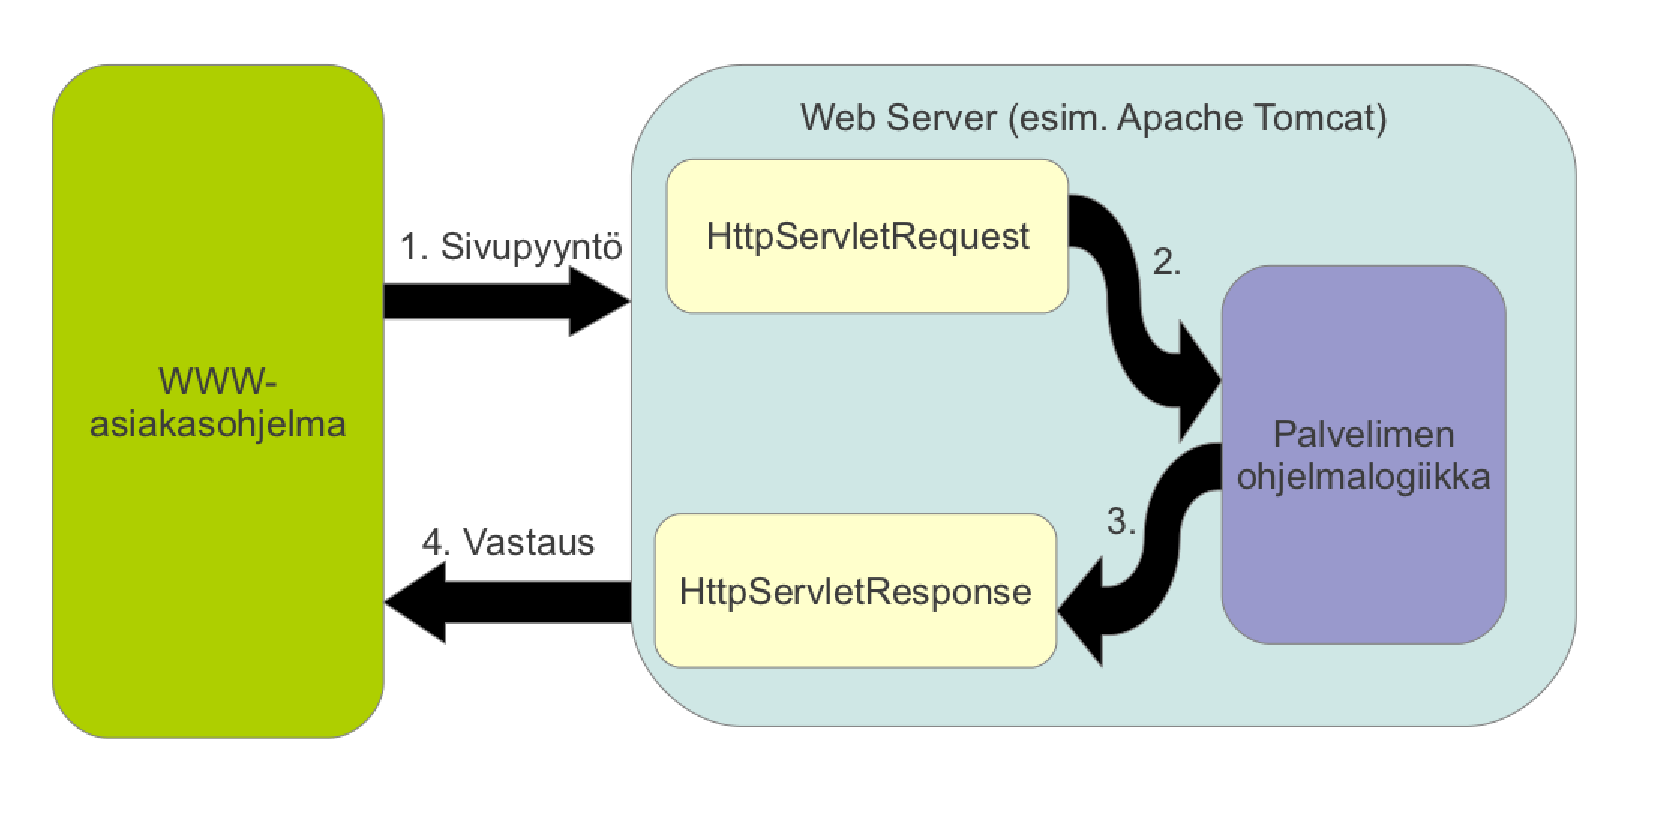
\includegraphics[width=\textwidth]{web/servlet.eps}
\caption{Kontrollin kulku Java Servlet-palvelimessa \cite{j2ee}.}%
\label{servlet}
\end{figure}

Servlettien jälkeen paljon suosiota on saanut CGI:stä kehittynyt FastCGI-protokolla, joka korjaa CGI:ssä havaittuja puutteita \cite{fastcgi}. Tällöin web-palvelin ei käynnistä jokaista pyyntöä kohti uutta palvelinprosessia, vaan pyynnöt lähetetään ja vastaanotetaan pistokkeen (socket) avulla palvelimella pyöriville prosesseille, jotka voivat palvella montaa pyyntöä yhtä aikaa. FastCGI-ohjelmat voivat olla myös hajautettu eri palvelimille, jolloin pyyntöjen välitykseen käytetään TCP-yhteyttä. FastCGI:tä voidaan käyttää minkä tahansa kielen kanssa, joka tukee pistokkeiden käyttöä. Näin ollen se on varteenotettava tekniikka web-sovellusten toteuttamiseen, koska ohjelmointikieli ei ole rajattu vain Javaan, vaan käytössä on useiden muiden kielten kirjo (esimerkiksi PHP, Python ja Ruby) \cite{fastcgi}.

Tiivistetysti web-sovellusten historiasta voidaan sanoa, että niistä on kehittynyt yksittäisistä palvelinprosesseista itsenäisiä ohjelmia, joita suoritetaan jatkuvasti palvelimella. Ohjelmat saavat kontrollin web-palvelimelta joko laajentamalla web-palvelimen toimintaa (Servlet, WEBrick yms) tai pistokkeiden avulla (FastCGI). Web-so\-vel\-luk\-set tuottavat käyttäjän syötteen ja web-sovelluksen sen hetkisen tilan mukaan käyttäjälle dynaamisen HTML-muotoisen sivun.